\chapter{定态微扰论与变分法}\label{chp:06}
% \makebox[5em][s]{} % 短题目拉间距

在量子力学中,薛定谔方程能够精确求解的情形不多,因此近似方法具有特殊的重要性.本章介绍处理定态问题的两种主要近似方法,即定态微扰论与变分法.半个多世纪以来,量子力学在应用方面已经有了许多进展,这些近似方法也有了许多发展、限于篇幅,我们只能对这些方法作初步介绍.

% 非简并态微扰论
\section[非简并态微扰论]{非简并态微扰论} \label{sec:06.01} % 
% \makebox[5em][s]{} % 短题目拉间距

研究一个物理体系,基本问题之一是求解能量本征方程
\begin{empheq}{equation}\label{eq61.1}
	\hat{H}\varPsi=E\varPsi
\end{empheq}
求出束缚态波函数和能级.如精确求解有困难,在下述前提下可以用微扰论方法求近似解.前提是:能量算符$\hat{H}$可以分解成大、小两项,
\begin{empheq}{equation}\label{eq61.2}
	\hat{H}=\hat{H}_{0}+\hat{H}^{\prime}
\end{empheq}
$\hat{H}_{0}$和$\hat{H}^{\prime}$均为厄密算符,按量级说$H^{\prime}\leqslant H_{0}$,而且$\hat{H}_{0}^{\prime}$的本征函数和本征值是已知的,或可以求出的.$H_{0}$称为零级能量(算符),$H^{\prime}$称为微扰.

$\hat{H}_{0}^{\prime}$的正交归一化本征函数记为$\varPsi_{k}^{(0)}$,$k=1,2,\cdots,n,\cdots$是编号数,与$\varPsi_{k}^{(0)}$相应的本征值记为$E_{k}^{(0)}$.$\varPsi_{k}^{(0)}$满足本征方程
\begin{empheq}{equation}\label{eq61.3}
	\hat{H}_{0}\varPsi_{k}^{(0)}=E_{k}^{(0)}\varPsi_{k}^{(0)}
\end{empheq}
及正交归一条件
\begin{empheq}{equation}\label{eq61.4}
	\langle \varPsi_{n}^{(0)}|\varPsi_{k}^{(0)} \rangle =\int\varPsi_{n}^{(0)*}\varPsi_{k}^{(0)}d\tau=\delta_{nk}
\end{empheq}
如果有几个本征函数相应于同一个能级$E_{k}^{(0)}$,这个能级称为简并能级,相应的那些本征态称为简并态.如果某个能级$E_{n}^{(0)}$只有一个相应的本征函数$\varPsi_{n}^{(0)}$,则称为非简并能级和非简并态.$\hat{H}_{0}$的全部本征态中,可能有一些是非简并态,其余则是简并态.例如氢原子(不考虑电子的自旋),基态$\varPsi_{100}$是非简并的,其他能量本征态$\varPsi_{nlm}(n\geqslant2)$都是简并态.在以下的叙述中,假定着重讨论的那个能级$(E_{n})$是非简并的.

回到\eqref{eq61.1}式的求解.由于$\hat{H}$中存在微扰$\hat{H}^{\prime}$,原来的($H_{0}$的)能级$E_{n}^{(0)}$将变成$E_{n}$,本征函数$\varPsi_{n}^{(0)}$将变成$\varPsi_{n}$,并满足\eqref{eq61.1}式,即
\begin{empheq}{equation*}\label{eq61.1'}
	(\hat{H}_{0}+\hat{H}^{\prime})\varPsi_{n}=E_{n}\varPsi_{n}
	\tag{$6.1.1^{\prime}$}
\end{empheq}
由于$H^{\prime}\leqslant H_{0}$,且与$E_{n}^{(0)}$将只有微小的差别,也与$\varPsi_{n}^{(0)}$也只有微小差别.为了求出$E_{n},\varPsi_{n}$,可设
\begin{empheq}{align}
	E_{n} &=E_{n}^{(0)}+E^{(1)}+E^{(2)}+\cdots	\label{eq61.5}\\
	\varPsi_{n} &=\varPsi_{n}^{(0)}+\varPsi^{(1)}+\varPsi^{(2)}	\label{eq61.6}
\end{empheq}
各项分别表示零级近似,一级修正,二级修正,等等,并规定各项的量级逐项相差$\frac{H^{\prime}}{H_{0}}$倍.关于\eqref{eq61.6}式,作如下规定.由于$\hat{H}_{0}$的全体本征函数$\{\varPsi_{k}^{(0)}\}$构成完备系,$\varPsi_{n}$可以展开成各$\varPsi_{k}^{(0)}$的线性叠加,
\begin{empheq}{equation*}
	\varPsi_{n}=\sum_{k}C_{k}\varPsi_{k}^{(0)}
\end{empheq}
暂不要求$\varPsi_{n}$是归一化的,则上式中总有一个系数(只要不为0)可以任意选择.为了方便,取$C_{n}=1$,则$\varPsi_{n}$的展开式为
\begin{empheq}{equation}\label{eq61.7}
	\varPsi_{n}=\varPsi_{n}^{(0)}+\sum_{k}^{\prime}C_{k}\varPsi_{k}^{(0)}
\end{empheq}
其中$\sum_{k}^{\prime}$表示对$k$求和,但$k\neq n$.这样做相当于规定\eqref{eq61.6}式中各个修正项中不含$\varPsi_{n}^{(0)}$项,因此这些修正项均与零级近似项正交,即
\begin{empheq}{equation}\label{eq61.8}
	\langle \varPsi_{n}^{(0)}|\varPsi^{(s)} \rangle =\int\varPsi_{n}^{(0)*}\varPsi^{(s)}d\tau=0,\quad s=1,2,\cdots
\end{empheq}
这个条件可以简化计算.将\eqref{eq61.5},\eqref{eq61.6}式代入\eqref{eq61.1'}式,并将各项按量级分开,可得:

\begin{subequations}\label{eq61.9}
	\eqindent{7}
	\begin{align}
	\shortintertext{零级项}
		(\hat{H}_{0}&-E_{n}^{(0)})\varPsi_{n}^{(0)}=0	\label{eq61.9a}\\
	\shortintertext{一级项}
		(\hat{H}_{0}-E_{n}^{(0)})&\varPsi^{(1)}=(E^{(1)}-\hat{H}^{\prime})\varPsi_{n}^{(0)}	\label{eq61.9b}\\
	\shortintertext{二级项}
		(\hat{H}_{0}-E_{n}^{(0)})\varPsi^{(2)}&=(E^{(1)}-\hat{H}^{\prime})\varPsi^{(1)}+E^{(2)}\varPsi_{n}^{(0)}	\label{eq61.9c}
	\end{align}\eqnormal
\end{subequations}
等等.\eqref{eq61.9a}式即\eqref{eq61.3}式$k=n$的情形.以$\varPsi_{n}^{(0)*}$左乘\eqref{eq61.9b}式,并对全空间积分,左端贡献为0,因此得到
\begin{empheq}{equation}\label{eq61.10}
	E^{(1)}=\int\varPsi_{n}^{(0)*}\hat{H}^{\prime}\varPsi_{n}^{(0)}d\tau=\langle \varPsi_{n}^{(0)}|\hat{H}^{\prime}|\varPsi_{n}^{(0)} \rangle \equiv H_{nn}^{\prime}
\end{empheq}
这就是能级$E_{n}$的一级修正项公式,$H_{nn}^{\prime}$的意义是微扰$H^{\prime}$在零级近似波函数$\varPsi_{n}^{(0)}$中的平均值对\eqref{eq61.9c}式作同样的处理,并注意到正交条件\eqref{eq61.8},可得
\begin{empheq}{equation}\label{eq61.11}
	E^{(2)}=\int\varPsi_{n}^{(0)*}\hat{H}^{\prime}\varPsi_{n}^{(1)}d\tau=\langle \varPsi_{n}^{(0)}|\hat{H}^{\prime}|\varPsi_{n}^{(1)} \rangle
\end{empheq}
但这还不是$E^{(2)}$的明显表示式,因为$\varPsi^{(1)}$尚未求出,设
\begin{empheq}{equation}\label{eq61.12}
	\varPsi^{(1)}=\sum_{k}^{\prime}C_{k}^{(1)}\varPsi_{k}^{(0)}
\end{empheq}
代入\eqref{eq61.9b}式,再用$\varPsi_{k}^{(0)*}$左乘全式,对全空间积分,并利用正交归一条件,可得
\begin{empheq}{equation}\label{eq61.13}
	C_{k}^{(1)}=\frac{H_{kn}^{\prime}}{E_{n}^{(0)}-E_{k}^{(0)}}
\end{empheq}
其中
\begin{empheq}{equation}\label{eq61.14}
	H_{kn}^{\prime}\equiv\int\varPsi_{k}^{(0)}\hat{H}^{\prime}\varPsi_{n}^{(0)}d\tau=\langle \varPsi_{k}^{(0)}|\hat{H}^{\prime}|\varPsi_{n}^{(0)} \rangle 
\end{empheq}
将\eqref{eq61.13}式代入\eqref{eq61.12}式,即得$\varPsi^{(1)}$的表示式
\begin{empheq}{equation}\label{eq61.15}
	\varPsi^{(1)}=\sum_{k}^{\prime}\frac{H_{kn}}{E_{n}^{(0)}-E_{k}^{(0)}}\varPsi_{k}^{(0)}
\end{empheq}
再代入\eqref{eq61.11}式, 即得
\begin{empheq}{equation}\label{eq61.16}
	E^{(2)}=\sum_{k}^{\prime}\frac{H_{nk}^{\prime}H_{kn}^{\prime}}{E_{n}^{(0)}-E_{k}^{(0)}}=\sum_{k}^{\prime}\frac{|H_{kn}^{\prime}|^{2}}{E_{n}^{(0)}-E_{k}^{(0)}}
\end{empheq}
用微扰论处理问题,通常的要求是,能级和波函数均应计算到第一个不等于零的修正项为止.对于波函数,由\eqref{eq61.15}式表示的一级修正总是不等于零的,一般不必再计算二级修正.对于能级,由于对称性等原因,$E^{(1)}$常常等于零,这时必须计算二级修正$E^{(2)}$.综合\eqref{eq61.5},\eqref{eq61.6},\eqref{eq61.10},\eqref{eq61.15},\eqref{eq61.16}式,可得准确到一级修正项的能量本征函数和准确到二级修正项的能级公式为
\eqlong
\begin{empheq}[box=\widefbox]{align}
	\varPsi_{n}&\approx\varPsi_{n}^{(0)}+\sum_{k}^{\prime}\frac{H_{kn}^{\prime}}{E_{n}^{(0)}-E_{k}^{(0)}}\varPsi_{k}^{(0)}		\label{eq61.17}	\\
	E_{n}&\approx E_{n}^{(0)}+H_{nn}^{\prime}+\sum_{k}^{\prime}\frac{|H_{kn}^{\prime}|^{2}}{E_{n}^{(0)}-E_{k}^{(0)}}		\label{eq61.18}
\end{empheq}\eqnormal


微扰论公式成立的条件为$|\varPsi^{(1)}|\leqslant|\varPsi_{n}^{(0)}|$,即
\begin{empheq}{equation}\label{eq61.19}
	|H_{kn}^{\prime}|\leqslant|E_{n}^{(0)}-E_{k}^{(0)}|,\quad k=1,2,\cdots
\end{empheq}
因此在能级密集的区域,微扰论的适用性稍差.

\example 一维谐振子,能量算符为
\begin{empheq}{equation*}
	H_{0}=-\frac{\hbar^{2}}{2m}\frac{d^{2}}{dx^{2}}+\frac{1}{2}m\omega^{2}x^{2}
\end{empheq}
设这谐振子受到微扰作用(另一种弹性力),
\begin{empheq}{equation*}
	H^{\prime}=\frac{\lambda}{2}m\omega^{2}x^{2},\quad |\lambda|\leqslant 1
\end{empheq}
试用微扰论公式计算能级的变化,并与精确解比较.

\solution $H_{0}$的本征函数记为$\varPsi_{n}^{(0)}$,这就是$\S$\ref{sec:02.05}讨论过的谐振子本征态.在表象中,(以$\varPsi_{n}^{(0)}$作为基矢)$x$的矩阵元只有下列类型不等于零:
\begin{empheq}{equation*}
	x_{n+1,n}=x_{n,n+1}=\bigg(\frac{n+1}{2}\frac{\hbar}{m\omega}\bigg)^{\frac{1}{2}}
\end{empheq}
因此,对于微扰$H^{\prime}$,它的矩阵元中不等于零的类型有
\begin{empheq}{align*}
	H_{nn}^{\prime} &=\frac{\lambda}{2}m\omega^{2}(x^{2})_{nn}=\frac{\lambda}{2}m\omega^{2}\sum_{k}x_{nk}x_{kn}	\\
	&=\frac{\lambda}{2}m\omega^{2}(|x_{n,n+1}|^{2}+|x_{n,n-1}|^{2})	\\
	&=\frac{1}{2}\bigg(n+\frac{1}{2}\bigg)\lambda\hbar\omega=\frac{\lambda}{2}E_{n}^{(0)}
	\\
	H_{n,n+2}^{\prime}&=H_{n+2,n}^{\prime}=\frac{\lambda}{2}m\omega^{2}x_{n,n+1}x_{n+1,n+2}	\\
	&=\frac{1}{4}\sqrt{(n+1)(n+2)}\lambda\hbar\omega
\end{empheq}
其中$E_{n}^{(0)}=\bigg(n+\frac{1}{2}\bigg)\hbar\omega$加是微扰前的能级.按照微扰论公式\eqref{eq61.10},\eqref{eq61.16}能级的一级修正和二级修正分别为
\begin{empheq}{align*}
	E_{n}^{1}&=H_{nn}^{\prime}=\frac{1}{2}\bigg(n+\frac{1}{2}\bigg)\lambda\hbar\omega	\\
	E_{n}^{(2)}&=\sum_{k}^{\prime}\frac{|H_{kn}^{\prime}|^{2}}{E_{n}^{(0)}-E_{k}^{(0)}}=\frac{1}{2\hbar\omega}(|H_{n-2,n}^{\prime}|^{2}-|H_{n+2,n}^{\prime}|^{2})	\\
	&=-\frac{1}{8}\bigg(n+\frac{1}{2}\bigg)\lambda^{2}\hbar\omega
\end{empheq}

本题显然可以精确求解,因为微扰后总能量算符为
\begin{empheq}{align*}
	H&=H_{0}+H^{\prime}=-\frac{\hbar^{2}}{2m}\frac{d^{2}}{dx^{2}}+\frac{1}{2}(1+\lambda)m\omega^{2}x^{2}	\\
	&=-\frac{\hbar^{2}}{2m}\frac{d^{2}}{dx^{2}}+\frac{1}{2}m\omega^{\prime2}x^{2},\quad \omega^{\prime}=\omega\sqrt{1+\lambda}
\end{empheq}
仍是谐振子问题.能级为
\begin{empheq}{equation*}
	E_{n}=\bigg(n+\frac{1}{2}\bigg)\hbar\omega^{\prime}=\bigg(n+\frac{1}{2}\bigg)\sqrt{1+\lambda}\hbar\omega
\end{empheq}
如将$\sqrt{1+\lambda}$展开成$\lambda$的幕级数,
\begin{empheq}{equation*}
	\sqrt{1+\lambda}=1+\frac{\lambda}{2}-\frac{\lambda^{2}}{8}+\cdots
\end{empheq}
则
\begin{empheq}{equation*}
	E_{n}=\bigg(n+\frac{1}{2}\bigg)\hbar\omega+\frac{\lambda}{2}\bigg(n+\frac{1}{2}\bigg)\hbar\omega-\frac{\lambda^{2}}{8}\bigg(n+\frac{1}{2}\bigg)\hbar\omega
\end{empheq}
准确到$\lambda^{2}$项,刚好和上述微扰论结果符合.







% 简并态微扰论
\section[简并态微扰论]{简并态微扰论} \label{sec:06.02} % 
% \makebox[5em][s]{} % 短题目拉间距

非简并态微扰论的特点是,受微扰作用后,原来的($\hat{H}_{0}$的)能级与本征函数都只发生微小的变化,$\varPsi_{n}^{(0)}\rightarrow\varPsi_{n}$,$E_{n}^{(0)}\rightarrow E_{n}$.简并态就不同,在微扰作用下,能级将发生分裂.

仍设$\hat{H}=\hat{H_{0}}+\hat{H}^{\prime}$,$\hat{H}^{\prime}$是微扰,设$\hat{H_{0}}$的某个能级$E_{n}^{(0)}$是$f$重简并的,有$f$个互相独立并且正交归一化的本征函数,
\begin{empheq}{equation}\label{eq62.1}
	\hat{H_{0}}\varPsi_{n\alpha}^{(0)}=E_{n}^{(0)}\varPsi_{n\alpha}^{(0)},\quad \alpha=1,2,\cdots,f
\end{empheq}
微扰$H^{\prime}$的存在一般地将引起这些本征态之间的耦合,因此,求解总能量的本征方程
\begin{empheq}{equation}\label{eq62.2}
	\hat{H}\varPsi_{n}=(\hat{H_{0}}+\hat{H}^{\prime})\varPsi_{n}=E_{n}\varPsi_{n}
\end{empheq}
时,$\varPsi_{n}$的零级近似一般应该是$\varPsi_{n\alpha}^{(0)}$的线性叠加,
\begin{empheq}{equation}\label{eq62.3}
	\varPsi_{n}^{(0)}=\sum_{\alpha}C_{\alpha}^{(0)}\varPsi_{n\alpha}^{(0)}
\end{empheq}
$\varPsi_{n}$的各级微扰修正仍记为$\varPsi^{(1)}$,$\varPsi^{(2)}$,$\cdots$,能级$E_{n}$的各级修正仍记为$E^{(1)}$,$E^{(2)}$,$\cdots$,即设
\begin{empheq}{align}
	\varPsi_{n}=\varPsi_{n}^{(0)}+\varPsi^{(1)}+\varPsi^{(2)}+\cdots	\label{eq62.4}\\
	E_{n}=E_{n}^{(0)}+E^{(1)}+E^{(2)}+\cdots		\label{eq62.5}
\end{empheq}
和上节一样,仍规定$\varPsi^{(1)}$,$\varPsi^{(2)}$,$\cdots$等不含$\varPsi_{n\alpha}^{(0)}$项,因此它们均和$\varPsi_{n\alpha}^{(0)}$正交,即
\begin{empheq}{align}\label{eq62.6}
	\langle \varPsi_{n\alpha}^{(0)}|\varPsi^{(1)} \rangle =0,\quad \langle \varPsi_{n\alpha}^{(0)}|\varPsi^{(2)} \rangle=0,\cdots
\end{empheq}
$\hat{H_{0}}$的其他($E_{n}^{(0)}$以外的)能级仍记为$E_{k}^{(0)}$,本征函数(不论是否简并)记为$\varPsi_{k}^{(0)}$
\begin{empheq}{equation}\label{eq62.7}
	\varPsi^{(1)}=\sum_{k}^{\prime}C_{k}^{(1)}\varPsi_{k}^{(0)}
\end{empheq}
将\eqref{eq62.4}、\eqref{eq62.5}式代入能量本征方程\eqref{eq62.2},并将各项按量级分开,形式上仍得到\eqref{eq61.9}列式,但必须牢记,现在由\eqref{eq61.3}式表示,它是$f$个简并态的线性叠加.

为了求出\eqref{eq62.3}式中各系数$C_{\alpha}^{(0)}$,以及能级的一级修正$E^{(1)}$,以各$\varPsi_{n\alpha}^{(0)*}(\alpha=1,2,\cdots,f)$轮流地左乘\eqref{eq61.9b}式,并对全空间积分,考虑到正交条件\eqref{eq62.6}式,即可得到下列关于$C_{\alpha}^{(0)}$的方程组:
\eqllong
\begin{empheq}{equation}\label{eq62.8}
	\begin{aligned}
		\begin{dcases}
			(H_{11}^{\prime}-E^{(1)})C_{1}^{(0)}+H_{12}^{\prime}C_{2}^{(0)}+\cdots+H_{1f}^{\prime}C_{f}^{(0)}=0	\\
			H_{21}^{\prime}C_{1}^{(0)}+(H_{22}^{\prime}-E^{(1)})C_{2}^{(0)}+\cdots+H_{2f}^{\prime}C_{f}^{(0)}=0	\\
			\qquad\qquad\qquad\quad\cdots\cdots\cdots\cdots	\\
			H_{f1}^{\prime}C_{1}^{(0)}+H_{f2}^{\prime}C_{2}^{(0)}+\cdots+(H_{ff}^{\prime}-E^{(1)})C_{f}^{(0)}=0
		\end{dcases}
	\end{aligned}
\end{empheq}\eqnormal
其中
\begin{empheq}{align}\label{eq62.9}
	H_{\alpha\beta}^{\prime}&\equiv H_{n\alpha,n\beta}=\int\varPsi_{n\alpha}^{(0)*}\hat{H}^{\prime}\varPsi_{n\beta}^{(0)}d\tau	\nonumber\\
	&=\langle \varPsi_{n\alpha}^{(0)}|\hat{H}^{\prime}|\varPsi_{n\beta}^{(0)} \rangle 
\end{empheq}
注意,\eqref{eq62.8}式中只出现$\{\varPsi_{n\alpha},\alpha=1,2,\cdots,f\}$子态矢空间中$\hat{H}^{\prime}$的矩阵元.实际上,\eqref{eq62.8}式相当于这子空间中微扰$\hat{H}^{\prime}$的本征方程,即
\eqlong
\begin{empheq}{equation*}\label{eq62.8'}
\begin{bmatrix}
	H_{11}^{\prime} & H_{12}^{\prime} & \cdots & H_{1f}^{\prime}	\\
	H_{21}^{\prime} & H_{22}^{\prime} & \cdots & H_{2f}^{\prime}	\\
	     \vdots     &      \vdots     &        & \vdots				\\
	H_{f1}^{\prime} & H_{f2}^{\prime} & \cdots & H_{ff}^{\prime}	\\
\end{bmatrix}\begin{bmatrix}
	C_{1}^{(0)}	\\	C_{2}^{(0)}	\\	\vdots	\\	C_{f}^{(0)}	\\
\end{bmatrix}=E^{(1)}\begin{bmatrix}
	C_{1}^{(0)}	\\	C_{2}^{(0)}	\\	\vdots	\\	C_{f}^{(0)}	\\
\end{bmatrix}
\end{empheq}
按照线性代数理论,\eqref{eq62.8}式存在非平庸解($C_{\alpha}^{(0)}$不全为0)的充要条件是
\begin{empheq}{equation}\label{eq62.10}
\begin{vmatrix}
	H_{11}^{\prime}-E^{(1)}	& H_{12}^{\prime} & \cdots & H_{1f}^{\prime}	\\
	H_{21}^{\prime}	& H_{22}^{\prime}--E^{(1)} & \cdots & H_{2f}^{\prime}	\\
	     \vdots     &      \vdots     &        & \vdots				\\
	H_{f1}^{\prime}	& H_{f2}^{\prime} & \cdots & H_{ff}^{\prime}-E^{(1)}	\\
\end{vmatrix}=0
\end{empheq}\eqnormal
亦即在$|\varPsi_{n\alpha}^{(0)}|$子空间中
\eqshort
\begin{empheq}{equation*}\label{eq62.10'}
	\det|H^{\prime}-E^{(1)}|=0
\end{empheq}
\eqref{eq62.10}式是$E^{(1)}$的$f$次代数方程,原则上可以求得$f$个$E^{(1)}$值,亦即原来的简并能级$E_{n}^{(0)}$在微扰论一级近似下已经分裂成为一组互相接近的能级.如\eqref{eq62.10}式的$f$个根互不重合,这表明在一级近似下能级$E_{n}^{(0)}$的简并化已经全部消除;如\eqref{eq62.10}式有重根,则表示简并化只是部分地消除.将由\eqref{eq62.10}式解出的每一个$E^{(1)}$值代回\eqref{eq62.8}式,求出$C_{\alpha}^{(0)}(\alpha=1,2,\cdots,f)$,并将其归一化,再代入\eqref{eq62.3}式,就得到和这个$E^{(1)}$相应的零级近似波函数.

有一种重要情况值得特别指出.如上述$f$个简并态中有一个特殊的$\varPsi_{n\beta}^{(0)}$,它与其他$\varPsi_{n\alpha}^{(0)}$构成的微扰矩阵元全部等于零,即$H_{\alpha\beta}^{\prime}=0$,则\eqref{eq62.8}式中唯一出现$C_{\beta}^{(0)}$的式子是
\begin{empheq}{equation*}
	(H_{\beta\beta}^{\prime}-E^{(1)})C_{\beta}^{(0)}=0
\end{empheq}\eqnormal
这时\eqref{eq62.8}式显然有特解
\begin{empheq}{equation*}
	E^{(1)}=H_{\beta\beta}^{\prime},\quad C_{\beta}^{(0)}=1,\quad C_{\alpha}^{(0)}=0(\alpha\neq\beta)
\end{empheq}
亦即$\varPsi_{n\beta}^{(0)}$单独构成正确的零级波函数,$E^{(1)}$等于微扰$H^{\prime}$的平均值.处理简并态微扰论问题,首先应该找出(如果有的话)这种特殊状态,问题就可得到简化.

波函数的一级修正$\varPsi^{(1)}$和能级的二级修正$E^{(2)}$也可以仿照$\S$\ref{sec:06.01}的程序而求出.$E^{(2)}$仍由\eqref{eq61.11}式表示,即
\eqlong
\begin{empheq}{equation}\label{eq62.11}
	E^{(2)}=\int\varPsi_{n}^{(0)*}\hat{H}^{\prime}\varPsi^{(1)}d\tau=\langle \varPsi_{n}^{(0)}|\hat{H}^{\prime}|\varPsi^{(1)} \rangle 
\end{empheq}\eqnormal
$\varPsi^{(1)}$由\eqref{eq62.7}式表示,$C_{k}^{1}$的公式仍可仿照$\S$\ref{sec:06.01}的程序求得,
\eqindent{1}
\begin{empheq}{equation}\label{eq62.12}
	C_{k}^{(1)}=\frac{\langle \varPsi_{k}^{(0)}|\hat{H}^{\prime}|\varPsi_{n}^{(0)} \rangle }{E_{n}^{(0)}-E_{k}^{(0)}}=\frac{1}{E_{n}^{(0)}-E_{k}^{(0)}}\sum_{\alpha}C_{\alpha}^{(0)}\langle \varPsi_{k}^{(0)}|\hat{H}^{\prime}|\varPsi_{n\alpha}^{(0)} \rangle 
\end{empheq}\eqnormal	\eqlong
\begin{empheq}{align}\label{eq62.13}
	\varPsi^{(1)}&=\sum_{n}^{\prime}\frac{1}{E_{n}^{(0)}-E_{k}^{(0)}}\langle \varPsi_{k}^{(0)}|\hat{H}^{\prime}|\varPsi_{n}^{(0)} \rangle\varPsi_{k}^{(0)}	\nonumber\\
	&=\sum_{k}^{\prime}\frac{\varPsi_{k}^{(0)}}{E_{n}^{(0)}-E_{k}^{(0)}}\sum_{\alpha}C_{\alpha}^{(0)}\langle \varPsi_{k}^{(0)}|\hat{H}^{\prime}|\varPsi_{n\alpha}^{(0)} \rangle
\end{empheq}
矩阵元$\langle \varPsi_{n}^{(0)}|\hat{H}^{\prime}|\varPsi_{n\alpha}^{(0)}\rangle$表示$\varPsi_{n\alpha}^{(0)}$态与$\varPsi_{k}^{(0)}$态由于$\hat{H}^{\prime}$的作用而产生耦合,因此(一级近似)波函数中出现$\varPsi_{k}^{(0)}$项.

将\eqref{eq62.13}式代入\eqref{eq62.11}式,即可得出$E^{(2)}$的具体表示式:
\begin{empheq}{align}\label{eq62.14}
	E^{(2)}&=\sum_{n}^{\prime}\frac{1}{E_{n}^{(0)}-E_{k}^{(0)}}\langle \varPsi_{n}^{(0)}|\hat{H}^{\prime}|\varPsi_{k}^{(0)} \rangle\langle \varPsi_{k}^{(0)}|\hat{H}^{\prime}|\varPsi_{n}^{(0)} \rangle	\\
	&=\sum_{k}^{\prime}\frac{1}{E_{n}^{(0)}-E_{k}^{(0)}}\sum_{\alpha,\beta}C_{\alpha}^{(0)}C_{\beta}^{(0)*}H_{n\beta,k}H_{k,n\alpha}	\nonumber	%\tag{$6.2.14^{\prime}$}
\end{empheq}
上式表明,能级的二级微扰修正$E^{(2)}$来源于微扰$H^{\prime}$引起的$\varPsi_{n}^{(0)}$态与其他各能级态$\varPsi_{k}^{(0)}$的耦合,矩阵元$\langle \varPsi_{k}^{(0)}|\hat{H}^{\prime}|\varPsi_{n}^{(0)}\rangle$就代表这种耦合.由于$\varPsi_{n}^{(0)}$系由$f$个简并态$\varPsi_{n\alpha}^{(0)},\varPsi_{n\beta}^{(0)},\cdots$组成,因此具体表现为下列形式的耦合:
\begin{empheq}{equation*}
	\varPsi_{n\alpha}^{(0)}\stackrel{H^{\prime}}{——}\varPsi_{k}^{(0)}\stackrel{H^{\prime}}{——}\varPsi_{n\beta},\quad \alpha,\beta=1,2,\cdots,f
\end{empheq}\eqnormal
而对于非简并能级,与$E_{n}^{(0)}$相应的状态只有一个$\varPsi_{n}^{(0)}$,二级能量修正$E_{n}^{(2)}$相应于耦合$\varPsi_{n}^{(0)}-\varPsi_{k}^{(0)}-\varPsi_{n}^{(0)}$,$E_{k}^{(0)}\neq E_{n}^{(0)}$.

处理简并态微扰论问题,核心目标是弄清楚能级的分裂情况.如在一级近似下,能级已经分裂,简并已经消除,[与此相应,各个零级波函数$\varPsi_{n}^{(0)}$也可经由\eqref{eq62.8}式确定下来]一般就不必再计算能级的二级修正和波函数的一级修正.[如有必要,可按\eqref{eq62.13}、\eqref{eq62.14}式计算.]如在能量一级近似下,简并并未完全消除,则对于仍然简并的那些能级,零级波函数实际上无法经由\eqref{eq62.8}式而确定下来,因此\eqref{eq62.13}、\eqref{eq62.14}式实际上无法使用.这种情况下,需要重新处理,$\varPsi_{n}^{(0)}$将与$E^{(2)}$(甚至$E^{(3)}$,$\cdots$)同时求出,亦即能级分裂发生在高级近似下.

\example 研究氢原子的第二个能级在外电场中引起的分裂,即史塔克效应.(计算能级的一级修正,不考虑电子自旋.)

\solution 以$E_{n}^{(0)}$和$\varPsi_{nlm}^{(0)}$表示孤立氢原子的能级和能量本征态($H_{0},\boldsymbol{L}^{2},L_{z}$的共同本征态).能级$E_{n}^{(0)}$的简并度是$n^{2}$,第二个能级$E_{2}U(0)$共有4个本征态,$nlm$值为
\begin{empheq}{equation*}
	nlm=200,210,211,21-1
\end{empheq}
$\varPsi_{nlm}^{(0)}$可以表示成(参看$\S$\ref{sec:05.01},$\S$\ref{sec:05.04})
\begin{empheq}{equation*}
	\varPsi_{nlm}^{(0)}=R_{nl}(r)Y_{lm}(\theta,\varphi)
\end{empheq}
与本题有关的径向波函数只有2种,$R_{21}$及$R_{20}$,$Y_{lm}$则有4种,它们是
\begin{empheq}{align*}
	Y_{00}&=\sqrt{\frac{1}{4\pi}}	\\
	Y_{10}&=\sqrt{\frac{3}{4\pi}}\cos\theta=\sqrt{\frac{3}{4\pi}}\frac{z}{r}	\\
	Y_{11}&=-\sqrt{\frac{3}{8\pi}}\sin\theta e^{i\varphi}=-\sqrt{\frac{3}{8\pi}}\frac{x+iy}{r}	\\
	Y_{1-1}&=\frac{3}{8\pi}\sin\theta e^{-i\varphi}
\end{empheq}

将氢原子置于电场$\mathscr{E}$中,以电场方向作为$z$轴,则电场对电子的作用势为
\begin{empheq}{equation}\label{eq62.15}
	H^{\prime}=e\mathscr{E}\cdot\boldsymbol{r}=e\mathscr{E}z=e\mathscr{E}r\cos\theta
\end{empheq}
如电场强度$\mathscr{E}$不超过$10^{6}$\si{V/cm},则$H^{\prime}$的数量级为
\begin{empheq}{equation*}
	H^{\prime}<(10^{6}\si{eV/cm})(10^{-8}\si{cm})=10^{-2}\si{eV}
\end{empheq}
而电子能级间距为几个电子伏,所以$H^{\prime}$可以当作微扰.

由于$\hat{H}^{\prime}$和$\hat{L_{z}}$对易,$\hat{H}^{\prime}$作用于$\varPsi_{nlm}^{(0)}$的结果,$\hat{L_{z}}$的取值$(m\hbar)$不变.由于$\hat{H}^{\prime}$是奇宇称,所以在任何$\varPsi_{nlm}^{(0)}$态下$H^{\prime}$的平均值为0.这样一来,在上述4个简并态组成的子空间中,凡和(211)及(21-1)态有关的$H^{\prime}$矩阵元全部为0,也就是说,在波函数的零级近似中,$H^{\prime}$的作用并不能使(211)、(21-1)态与其他简并态发生耦合,它们就是正确的零级波函数,而且不受$H^{\prime}$影响,能级不发生变化(一级近似).

在$n=2$的上述态矢空间中,仅有的不等于零的$H^{\prime}$矩阵元是
\begin{empheq}{align*}
	H_{200,210}^{\prime}&=H_{210,200}^{\prime}=e\mathscr{E}\int z\varPsi_{200}\varPsi_{210}d\tau	\\
	&=\frac{e\mathscr{E}}{\sqrt{3}}\int_{0}^{\infty}r^{3}R_{20}R_{21}dr
\end{empheq}
径向波函数的具体函数形式见\eqref{eq54.27}、\eqref{eq54.28}式,经过简单计算,得到
\begin{empheq}{equation}\label{eq62.16}
	H_{200,210}^{\prime}=H_{210,200}^{\prime}=-3e\mathscr{E}a_{0}
\end{empheq}
$a_{0}=\frac{\hbar^{2}}{\mu\e^{2}}$是玻尔半径.读者如能注意到$Y_{lm}$和$H^{\prime}$在直角坐标系中的对称性(奇偶性),当能对上述关于$H^{\prime}$矩阵元的讨论加深印象.

至此,初步结论是,在外电场作用下,4个简并态中(211)态和(21-1)态并不与其他态耦合,能级仍保持原来的值.(200)态和(210)态则产生耦合,这将导致能级分裂.将简并态微扰论用于这两个简并态,令
\begin{empheq}{equation}\label{eq62.17}
	\varPsi_{n}^{(0)}=C_{1}^{(0)}\varPsi_{200}^{(0)}+C_{2}^{(0)}\varPsi_{210}^{(0)}
\end{empheq}
\eqref{eq62.8}式具体表现为
\begin{empheq}{equation}\label{eq62.18}
	{}\begin{dcases}
		E^{(1)}C_{1}^{(0)}+3e\mathscr{E}a_{0}C_{2}^{(0)}=0	\\
		3e\mathscr{E}a_{0}C_{1}^{(0)}+E^{(1)}C_{2}^{(0)}
	  \end{dcases}
\end{empheq}
\eqref{eq62.10}式表现为
\begin{empheq}{equation}\label{eq62.19}
	(E^{(1)})^{2}-(3e\mathscr{E}a_{0})^{2}=0
\end{empheq}
解为
\eqshort
\begin{empheq}{equation*}
	E^{(1)}=\pm3e\mathscr{E}a_{0}
\end{empheq}\eqnormal
此即能级$E_{2}^{(0)}$的一级微扰分裂(一级史塔克效应).再由\eqref{eq62.18}式可求出$C_{1}^{(0)}$,$C_{2}^{(0)}$,结果为
\eqllong
\begin{empheq}{equation}\label{eq62.20}
	\begin{aligned}
		E^{(1)}&=3e\mathscr{E}a_{0},\quad C_{1}^{(0)}=-C_{2}^{(0)},\quad 
		\varPsi^{(0)}=\frac{1}{\sqrt{2}}(\varPsi_{200}^{(0)}-\varPsi_{210}^{(0)})	\\
		E^{(1)}&=-3e\mathscr{E}a_{0},\quad C_{1}^{(0)}=C_{2}^{(0)},\quad 
		\varPsi^{(0)}=\frac{1}{\sqrt{2}}(\varPsi_{200}^{(0)}+\varPsi_{210}^{(0)})
	\end{aligned}
\end{empheq}\eqnormal
能级分裂如图\ref{fig.6-1}所示.

\begin{figure}[!h]
	\centering
	\small
	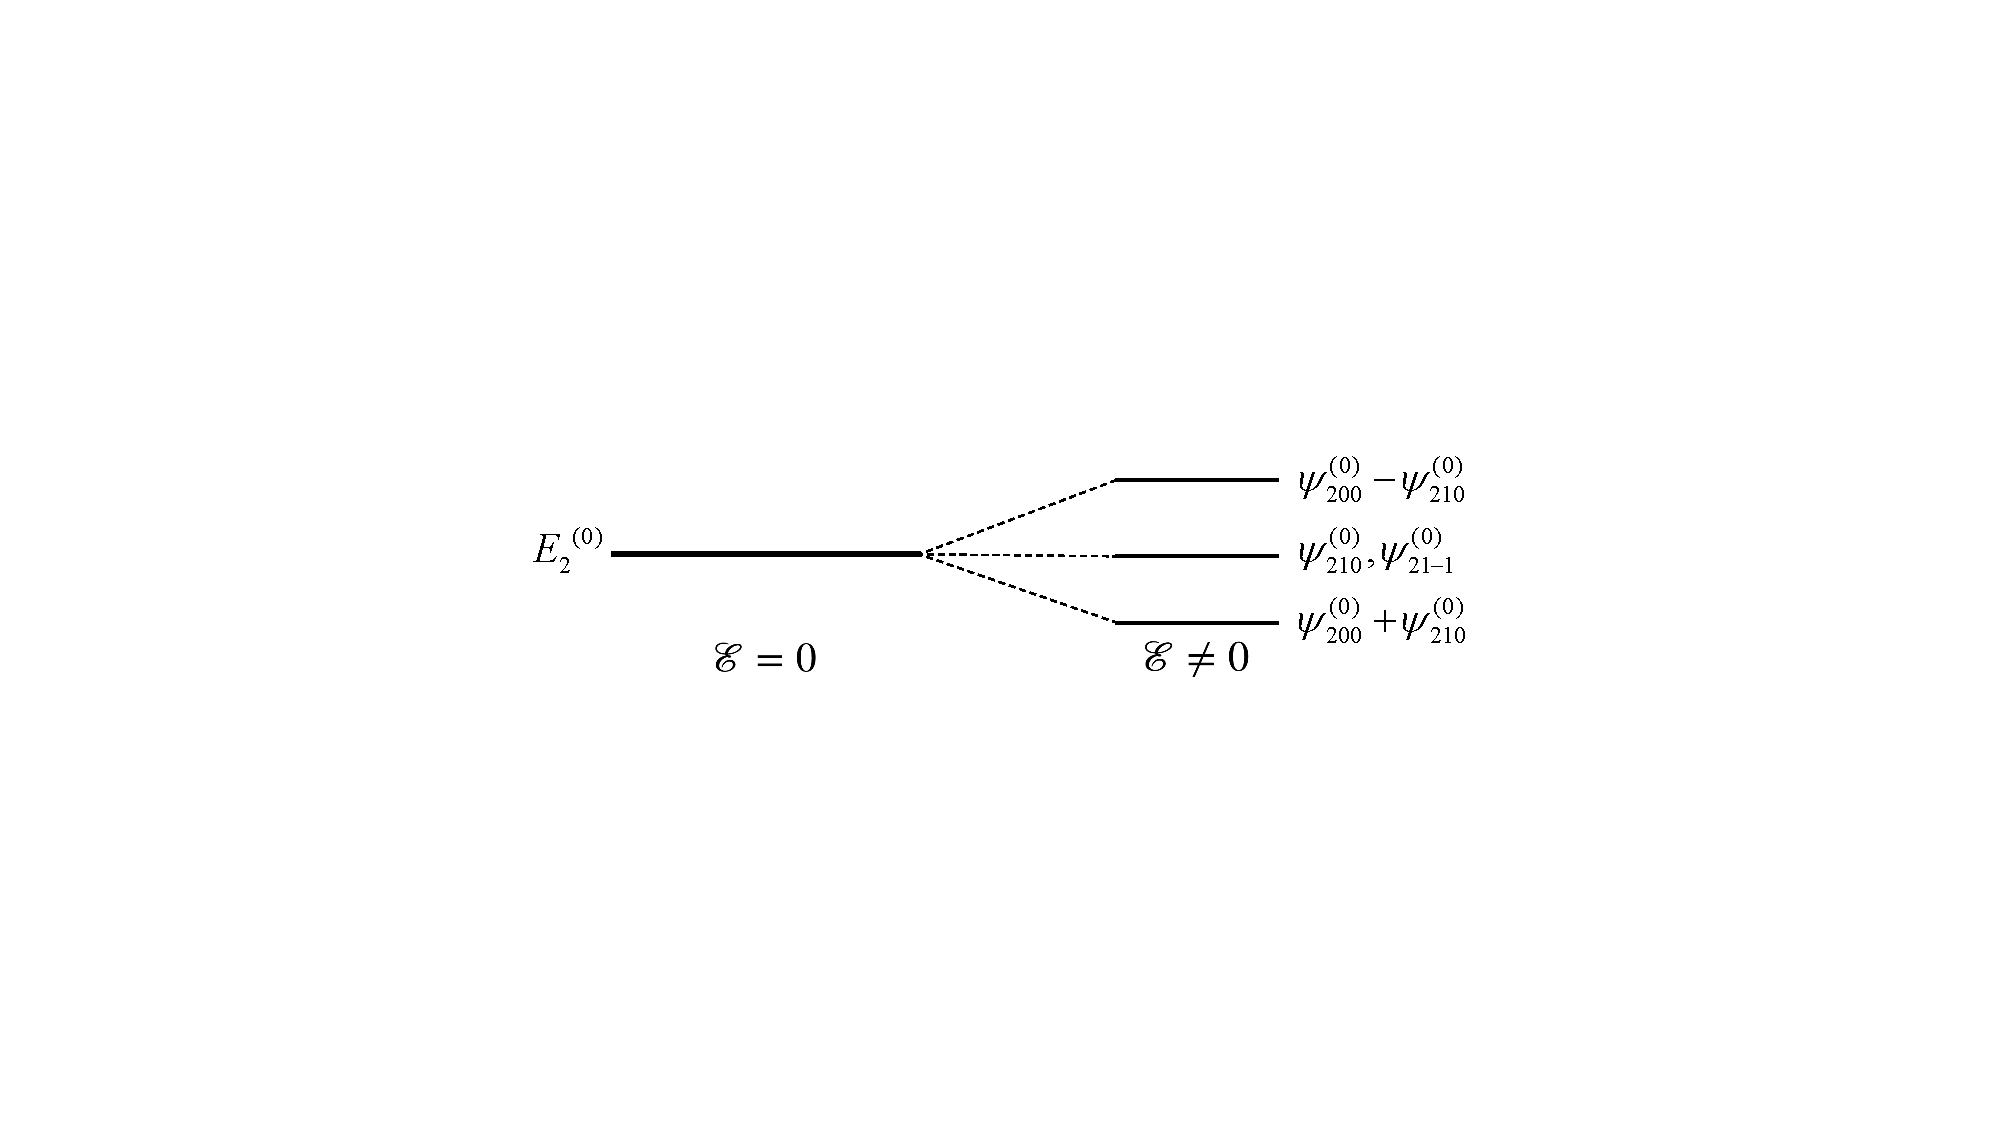
\includegraphics[width=6cm,clip]{QM file/figure/6-1}
	\caption{}\label{fig.6-1}
\end{figure}

值得注意的是原子的物理性质在外电场作用下发生的变化,氢原子的电偶极矩算符为
\eqshort
\begin{empheq}{equation}\label{eq62.21}
	\boldsymbol{D}=-e\boldsymbol{r}
\end{empheq}\eqnormal
未加电场时,原子的定态$\varPsi_{nlm}^{(0)}$均有或奇或偶的宇称,而$\boldsymbol{D}$为奇宇称,因此$\boldsymbol{D}$的平均值为0.在电场$\mathscr{E}$作用下,分裂出两个新的能级$E_{2}^{(0)}\pm3e\mathscr{E}a_{0}$,相应的波函数由\eqref{eq62.20}式表示,它们都是$\varPsi_{200}^{(0)}$和$\varPsi_{210}^{(0)}$的耦合态,已经没有宇称性,平均电矩也不为零,计算结果是
\eqlong
\begin{empheq}{align*}
	\varPsi^{(0)}&=\frac{1}{\sqrt{2}}(\varPsi_{200}^{(0)}-\varPsi_{210}^{(0)}),\quad \overline{D_{x}}=\overline{D_{y}}=0,\quad \overline{D_{z}}=-3ea_{0}	\\
	\varPsi^{(0)}&=\frac{1}{\sqrt{2}}(\varPsi_{200}^{(0)}+\varPsi_{210}^{(0)}),\quad \overline{D_{x}}=\overline{D_{y}}=0,\quad \overline{D_{z}}=3ea_{0}
\end{empheq}\eqnormal
正是耦合态的这个固有电矩在外电场中获得的势能
\begin{empheq}{equation*}
	E^{(1)}=0\langle \mathscr{E}\cdot\boldsymbol{D} \rangle=-\mathscr{E}\overline{D_{z}}=\pm3e\mathscr{E}a_{0}
\end{empheq}
造成了能级分裂.


% 变分法
\section[变分法]{变分法} \label{sec:06.03} % 
% \makebox[5em][s]{} % 短题目拉间距

考虑任一物理体系的束缚态,以$\hat{H}$表示体系的总能量算符($\hat{H}$与时间无关).任取一个归一化的波函数$\varPsi$(与时间无关),计算$\hat{H}$的平均值,并记为$E$,即
\begin{empheq}{align}
	&\int\varPsi^{*}\varPsi d\tau=\langle \varPsi|\varPsi \rangle =1		\label{eq63.1}\\
	E&=\int\varPsi^{*}\hat{H}\varPsi d\tau=\langle \varPsi|\hat{H}|\varPsi \rangle	\label{eq63.2}
\end{empheq}
然后令波函数作任意微小变化(变分)
\begin{empheq}{equation}\label{eq63.3}
	\varPsi\rightarrow\phi=\varPsi+\delta \varPsi
\end{empheq}
对于函数$\phi$重新计算$\hat{H}$的平均值,记为$E+\delta E$
\begin{empheq}{equation}\label{eq63.4}
	E+\delta E=\frac{\int\phi^{*}\hat{H}\phi d\tau}{\int\phi^{*}\phi d\tau}
\end{empheq}
(注意,$\phi$可能不再是归一化的)将\eqref{eq63.3}式代入\eqref{eq63.4}式,略去二级小量($\delta\varPsi$的二次项),得到如下结果:
\eqlong
\begin{empheq}{align*}
	\int\phi^{*}\phi d\tau &=1+\bigg(\int\varPsi\delta\varPsi^{*}d\tau+c.c \bigg)	\\
	\int\phi^{*}\hat{H}\phi d\tau&=\int(\varPsi^{*}+\delta\varPsi^{*})\hat{H}(\varPsi+\delta\varPsi)d\tau	\\
	&=E+\int\delta\varPsi^{*}\hat{H}\varPsi d\tau+\int\varPsi^{*}\hat{H}\delta\varPsi d\tau	\\
	&=E+\bigg(\int\delta\varPsi^{*}\hat{H}\varPsi d\tau+c.c \bigg)	\\
	&=E+\delta E+E\bigg(\int\varPsi\delta\varPsi^{*}d\tau+c.c\bigg)
\end{empheq}
即
\begin{empheq}{equation}\label{eq63.5}
	\delta E=\int\delta\varPsi^{*}\hat{H}\varPsi d\tau+c.c.-E\bigg(\int\delta\varPsi^{*}\varPsi d\tau+c.c \bigg)
\end{empheq}\eqnormal
考虑到$\delta\varPsi$的任意性,由\eqref{eq63.5}式容易看出以下结论:

(i) 如果$\varPsi$满足方程$\hat{H}\varPsi=E\varPsi$,则$\delta E=0$.

(ii) 如果对任意$\delta\varPsi$要求$\delta E=0$,则$\varPsi$必须满足
\eqshort
\begin{empheq}{equation}\label{eq63.6}
	\hat{H}\varPsi=E\varPsi
\end{empheq}\eqnormal
总之,“$\hat{H}$的平均值取变分极值$(\delta E=0)$”与“$\varPsi$为$\hat{H}$的本征函数”是等价的,这称为变分原理.

这个变分原理曾被薛定谔用来建立波动力学.本节向读者介绍一种寻找束缚态波函数与能级的近似方法,俗称变分法,它的理论基础就是上述变分原理.

设体系的总能量算符$\hat{H}$已经给定,但能量本征方程无法精确求解.设能级(按照由低到高的次序)为$E_{0},E_{1},E_{2},\cdots$相应的束缚态波函数(归一化的)为$\varPsi_{0}$,$\varPsi_{1}$,$\varPsi_{2}$,$\cdots$.任取一个归一化的波函数$\varPsi$,按照态叠加原理,$\varPsi$在原则上可以表示成能量本征函数的线性叠加:
\begin{empheq}{equation}\label{eq63.7}
	\varPsi=\sum_{n}C_{n}\varPsi_{n},\quad \sum_{n}C_{n}^{*}C_{n}=1
\end{empheq}
则在$\varPsi$态中$\hat{H}$的平均值(记为$E$)为
\begin{empheq}{equation}\label{eq63.8}
	E=\int\varPsi^{*}\hat{H}\varPsi d\tau=\sum_{n}C_{n}^{*}C_{n}E_{n}
\end{empheq}
由于$E_{n}\geqslant E_{0}$,显然$E\geqslant E_{0}$,$E_{0}$为基态能级.以上分析提示我们可以这样来寻找基态$\varPsi_{0}$,$E_{0}$.选取一种估计接近于基态的函数(归一化的)形式$\varPsi(\lambda,x)$,$x$代表坐标变量,$\lambda$为待定参数(一个或多个).对$\varPsi(\lambda,x)$计算$\hat{H}$的平均值,记为$E(\lambda)$,即
\begin{empheq}{equation}\label{eq63.9}
	E(\lambda)=\int\varPsi^{*}(\lambda,x)\hat{H}\varPsi(\lambda,x)d\tau
\end{empheq}
在不改变$\varPsi$的函数形式的条件下,根据变分极值条件
\begin{empheq}{equation}\label{eq63.10}
	\delta E=0,\quad \text{即}\frac{\partial E(\lambda)}{\partial\lambda}=0
\end{empheq}
求出$\lambda$的最佳值$\lambda_{0}$,相应的$\varPsi(\lambda_{0},x)$及$E(\lambda_{0}$即可作为基态波函数$\varPsi_{0}$及基态能级$E_{0}$的近似.如所得结果不够满意,可以另选一种$\varPsi$的函数形式,重复上述计算.在选择试探波函数$\varPsi(\lambda,x)$的函数形式时,当然应充分考虑基态的各方面性质,并可将其他近似方法(例如微扰论)求得的结果作为参考.一般说来,用这种参数变分法通常总能求得较好的结果,当然,计算工作量有时较大,需要电子计算机的帮助.

同样的方法也可用来寻找激发态$\varPsi_{n}$,$E_{n}$的近似,条件是所有能量小于$E_{n}$的能量本征态($\varPsi_{0}$,$\varPsi_{1}$,$\cdots$,$\varPsi_{n-1}$)均已求出,这时$\varPsi_{n}$的试探函数$\varPsi(\lambda,x)$应选取成与这些波函数正交,以保证在展开式\eqref{eq63.7}中没有这些状态的成分,则
\eqindent{7}
\begin{empheq}{align*}
	\varPsi&(\lambda,x)=C_{n}\varPsi_{n}+C_{n+1}\varPsi_{n+1}+\cdots	\\
	E(\lambda)&=C_{n}^{*}C_{n}E_{n}+C_{n+1}^{*}C_{n+1}E_{n+1}+\cdots\geqslant E_{n}
\end{empheq}\eqnormal
再用变分极值条件\eqref{eq63.10}式求出$\lambda$的最佳值$\lambda_{0}$,即可得到$\varPsi_{n}$,$E_{n}$的近似结果.

\example 粒子(质量$m$)在无限深势阱$(-a<x<a)$中运动.试用多项式近似结合变分法求基态能级的近似值,并与精确解比较.

\solution 精确解见$\S$\ref{sec:02.04},基态为(用本节的符号)
\begin{empheq}{equation}\label{eq63.11}
	\varPsi_{0}(x)=\sqrt{\frac{1}{a}}\cos\frac{\pi x}{2a},\quad E_{0}=\frac{\pi^{2}\hbar^{2}}{8ma^{2}}
\end{empheq}
$\varPsi_{0}$为偶宇称,并满足边界条件$\varPsi(a)=\varPsi(-a)=0$.

如用多项式作为$\varPsi_{0}$的近似表示,考虑到此为偶宇称,应取
\begin{empheq}{equation}\label{eq63.12}
	\varPsi=C_{0}+C_{2}\bigg(\frac{x}{a}\bigg)^{2}+C_{4}\bigg(\frac{x}{a}\bigg)^{4}+\cdots
\end{empheq}
如只取前两项,为了满足边界条件,必须取$C_{2}=-C_{0}$,而$C_{0}$可由归一化条件
\eqshort
\begin{empheq}{equation*}
	\int_{-a}^{a}\varPsi^{*}\varPsi dx=1
\end{empheq}
定出,结果为
\begin{empheq}{equation}\label{eq63.13}
	\varPsi=\sqrt{\frac{15}{16a}}\bigg(1-\frac{x^{2}}{a^{2}}\bigg)
\end{empheq}\eqnormal
这样已经不再有安插变分参数的余地.由\eqref{eq63.13}式求得能量平均值为
\eqlong
\begin{empheq}{equation}\label{eq63.14}
	E=\int_{-a}^{a}\varPsi^{*}\bigg(-\frac{\hbar^{2}}{2m}\frac{d^{2}}{dx^{2}}\bigg)\varPsi dx=\frac{5}{4}\frac{\hbar^{2}}{ma^{2}}
\end{empheq}\eqnormal
这和$E_{0}$的精确值已经相当接近,事实上
\begin{empheq}{equation*}
	E/E_{0}=10/\pi^{2}\approx\num{1.0132}
\end{empheq}

如取\eqref{eq63.12}式中前三项作为基态试探波函数,为了满足边界条件,应取$C_{4}=-(C_{0}+C_{2})$.如以$C_{0}$作为归一化系数,则试探波函数可以表示成
\eqlong
\begin{empheq}{equation}\label{eq63.15}
	\varPsi(\lambda,x)=C_{0}\bigg[1+\lambda\bigg(\frac{x}{a}\bigg)^{2}-(1+\lambda)\bigg(\frac{x}{a}\bigg)^{4}\bigg]
\end{empheq}\eqnormal
由归一化条件求出
\begin{empheq}{equation}\label{eq63.16}
	\frac{16}{315}(\lambda^{2}+8\lambda+28)aC_{0}^{2}=1
\end{empheq}
而能量平均值为
\eqlong
\begin{empheq}{align}\label{eq63.17}
	E(\lambda)&=-\frac{\hbar^{2}}{2m}\int_{-a}^{a}\varPsi(\lambda,x)\frac{d^{2}}{dx^{2}}\varPsi(\lambda,x)dx	\nonumber\\
	&=\frac{3}{4}\frac{11\lambda^{2}+36\lambda+60}{\lambda^{2}+8\lambda+28}\frac{\hbar^{2}}{ma^{2}}
\end{empheq}\eqnormal
根据变分极值条件\eqref{eq63.10}式,求得$\lambda$的最佳值为
\begin{empheq}{equation*}
	\lambda_{0}=-\num{1.22075},\quad \lambda_{0}^{\prime}=-\num{8.31775}
\end{empheq}
代入\eqref{eq63.17}式,得到
\eqlong
\begin{empheq}{equation}\label{eq63.18}
	E(\lambda_{0})=\num{1.23372}\frac{\hbar^{2}}{ma^{2}},\quad E(\lambda_{0}^{\prime})=\num{12.7663}\frac{\hbar^{2}}{ma^{2}}
\end{empheq}\eqnormal
$E(\lambda_{0})$和基态能级的精确值非常接近,事实上
\begin{empheq}{equation*}
	E_{0}=\frac{\pi^{2}}{8}\frac{\hbar^{2}}{ma^{2}}\approx \num{1.23370}\frac{\hbar^{2}}{ma^{2}}
\end{empheq}
\pskip
$E(\lambda_{0}^{\prime})$则接近于第三个能级$\frac{9\pi^{2}\hbar^{2}}{8ma^{2}}$.

将$\lambda_{0}=-\num{1.22075}$代入\eqref{eq63.15}式,所得波函数$\varPsi(\lambda_{0},x)$的波形非常接近于真正的基态$\varPsi_{0}$,计算表明
\begin{empheq}{equation*}
	\int_{-a}^{a}\varPsi_{0}\varPsi(\lambda_{0},x)dx=1-\alpha,\quad \alpha<10^{-5}
\end{empheq}
亦即$\varPsi(\lambda_{0},x)$中基态为主要成分,各种激发态成分之和仅为
\begin{empheq}{equation*}
	1-(1-\alpha)^{2}=2\alpha-\alpha^{2}\sim 10^{-5}.
\end{empheq}












% 习题
\begin{exercises}
	
\exercise 某物理体系只有两个能级.$H_{0}$在表象中$H$的矩阵表示为
\begin{empheq}{equation*}
	H=H_{0}+H^{\prime}=\begin{bmatrix}
		E_{1}^{(0)}+a & b \\
		b E_{2}^{(0)}+a	\\
	\end{bmatrix}
\end{empheq}
$a,b$为实数,并且远小于$(E_{2}^{(0)}-E_{1}^{(0)})$.试求能级的精确值.再按照微扰论公式写出能级(二级近似).比较两种结果.

\exercise 粒子在势阱
\begin{empheq}{equation*}
	{V(x)=}
	\begin{dcases}
		V_{0}x/a,\quad 0<x<a	\\
		\infty,\qquad x\leqslant0,x\geqslant a
	\end{dcases}
\end{empheq}
中运动,$V_{0}\leqslant\dfrac{\hbar^{2}}{m^{2}a}$,试用微扰论计算其能谱(一级近似).

[提示:利用无限深平底势阱(2-5题)的结果.]

\exercise 粒子在无限深势阱$(-a<x<a)$中运动.如受到微扰$H^{\prime}=\gamma\delta(x)$作用,求各能级产生的变化(一级修正).微扰论成立的条件是什么?

\exercise 三维自由转子的能量算符为$H_{0}=\dfrac{\boldsymbol{L}^{2}}{2\boldsymbol{I}}$,$\boldsymbol{I}$为转动惯量.试确定其能级及简并度.设此转子受到微扰$H^{\prime}=\lambda\cos\theta$作用,求基态能级的变化(二级近似).

\exercise 一维谐振子,受到微扰$H^{\prime}=\dfrac{\lambda p}{m}$作用,试按照微扰论公式求能谱(准确到$\lambda^{2}$),与精确值(3-30题)比较.

\exercise 三维各向同性谐振子,受到微扰
\begin{empheq}{equation*}
	H^{\prime}=\lambda xyz+\bigg(\frac{\lambda^{2}}{\hbar\omega}\bigg)x^{2}y^{2}z^{2}
\end{empheq}
作用,求基态能级,准确到$\lambda^{2}$.

[提示:采用直角坐标系,$\varPsi_{n_{1}n_{2}n_{3}}=\varPsi_{n1}(x)+\varPsi_{n2}(y)+\varPsi_{n3}(z)$].

\exercise 在类氢离子(核电荷$Ze$)的能谱计算中,通常视原子核为点电荷.这样求出的能级记成$E_{n}^{(0)}$.实际上原子核更接近于电荷均匀分布的小球,核半径$R=r_{0}Z^{1/3},r_{0}=\num{1.635}\times10^{-13}\si{cm}$.试求这种核电荷分布效应对于离子中电子基态能级的影响(一级微扰修正).

$\bigg[$提示:电子所受库仑作用势为
\begin{empheq}{equation*}
	{V(r)}
	\begin{dcases}
		-\frac{Z\e^{2}}{R}\bigg(\frac{3}{2}-\frac{r^{2}}{2R^{2}}\bigg),\quad r<R	\\
		-\frac{Z\e^{2}}{r},\qquad\quad \qquad\quad  r>R
	\end{dcases}
\end{empheq}
以$H^{\prime}=V(r)-\bigg(-\dfrac{Z\e^{2}}{r}\bigg)$作为微扰.注意$R\ll\dfrac{a_{0}}{Z}$.
$\bigg]$
\exercise 在静电场中,如点电荷获得的静电势能是$V(\boldsymbol{r})$,则将点电荷换成电荷均匀分布的小球(半径$r_{0}$)时,静电势能是
\begin{empheq}{equation*}
	U(\boldsymbol{r})=V(\boldsymbol{r})+\frac{1}{6}r_{0}^{2}\nabla^{2}V(\boldsymbol{r})+\cdots
\end{empheq}
其中$\boldsymbol{r}$为球心位置对于氢原子,(原子核即质子,视为点电荷)视电子为点电核时,库仑势能为$V(\boldsymbol{r})=-\dfrac{\ell^{2}}{r}$.如视电子为电荷均匀分布的小球,$r_{0}=\dfrac{\e^{2}}{m_{e}C^{2}}$(经典电子半径),库仑势能改为上述$U(\boldsymbol{r})$,求1s和2p能级的一级微扰修正.[相当于兰姆移位(Lamb shift)]

[提示:$H^{\prime}=V-V,\nabla^{2}\dfrac{1}{r}=-4\pi\delta(\boldsymbol{r})$]

\exercise 有一个在磁场中的三维转子,能量算符为
\begin{empheq}{equation*}
	H=k\boldsymbol{L}^{2}+\omega L_{z}+\lambda L_{x},\quad k,\omega\gg\lambda
\end{empheq}

(a) 视$\lambda$项为微扰,求能级的零级近似、一级修正、二级修正.

(b) 求能级的精确值,并与微扰论结果比较.

[提示:找一个方向$\boldsymbol{n}$,使$\omega L_{z}+\lambda L_{x}=\omega^{\prime}L_{n}$,而$\boldsymbol{L}^{2},L_{n}$有共同本征态,$L_{n}$本征值为$m\hbar$.]

\exercise (a) 粒子在二维无限深方势阱$(0<x<a,0<y<a$中运动,写出能级与能量本征函数.

(b) 加上微扰$H^{\prime}=\lambda xy$,求最低两个能级的一级微扰修正.

\exercise 苯分子的“自由电子模型”认为电子是在一个环形势场中运动,并受到具有$\ce{C_{6}}$对称性的微扰作用.即

(a) 不计及微扰作用时,可以认为电子是在半径为$R$的环上自由运动.写出能量本征值与本征函数,作为零级近似.(参看2-6题)

(b) 微扰可以表示成$H^{\prime}=V(\varphi)=-V_{0}\cos 6\varphi$,试研究它对各能级的影响(一级修正),特别要找出发生分裂的能级.

\exercise 对于类氢离子的第二个能级,讨论其在微扰$H^{\prime}=xyf(r)$作用下的分裂情况(一级效应).$f(r)$有良好的积分收敛性,无其他特殊性质.

\exercise 某体系的能量算符$H_{0}$只有两个本征值$E_{1}^{(0)}$,$E_{2}^{(0)}$,前者二重简并,后者不简并.受微扰$H^{\prime}$作用后,能量算符的矩阵表示($H_{0}$表象)为
\begin{empheq}{equation*}
	H=H_{0}+H^{\prime}=\begin{bmatrix}
		E_{1}^{(0)} & 0 & a	\\
		0 & E_{1}^{(0)} & b	\\
		a & b & E_{2}^{(0)}	\\
	\end{bmatrix}
\end{empheq}
试用微扰论求能级(二级近似).再用矩阵方法求能级的精确公式,然后作近似展开$(a,b\ll E_{2}^{(0)}\sim E_{1}^{(0)})$,与微扰论结果比较.

\exercise (a) 如粒子(质量$\mu$)的波函数(未归一化)为
\begin{empheq}{equation*}
	\varPsi(\lambda,r)=e^{-\lambda r}\quad\text{或}\quad e^{-\lambda^{2}r^{2}/2}
\end{empheq}
求动能平均值.

(b) 以这两种函数分别作为三维各向同性谐振子的基态试探函数($\lambda$为变分参数),求基态能级近似值.

\exercise 粒子(质量$\mu$)在势场$V(x)=kx^{4}(k>0)$中运动,用变分法求基态能级近似值.试探波函数(未归一化)取为

(a) $\varPsi(\lambda,x)=e^{-\lambda|x|}$

(b) $\varPsi(\lambda,x)=e^{-\lambda^{2}r^{2}/2}$.解释(a)项结果较差的原因.

\exercise 粒子在无限深势阱$(-a<x<a)$中运动,试用多项式近似及变分法求第一激发能级的近似值,与精确值比较.

$\bigg[$提示:波函数为奇宇称,取$\varPsi=N\biggl\{\dfrac{x}{a}+\lambda\bigg(\dfrac{x}{a}\bigg)^{3}-(1+\lambda)\bigg(\dfrac{x}{a}\bigg)^{5}\biggr\}.$	$\bigg]$

\end{exercises}
